\documentclass[paper.tex]{subfiles}

\begin{document}
\section{Introduction}
\label{sec:intro}

Quandles are algebraic structures that are deeply connected to knots. This connection is most strikingly presented by considering the strands of a knot diagrams as objects acted on by the operation of
undercrossing, $\uc$. A set of axioms that $\uc$ must satisfy in order to be a `knot diagram invariant' (in a sense we will define shortly) can be easily derived from the Reidemeister moves, as shown in
Section~\ref{sec:quandle_axioms}.

But this is not the only way that quandles can be seen to be deeply connected to knots - the fundamental group for a knot $K$, $\pi_1(\R^3 \setminus K)$ is a quandle!

\subsection{Notation}

We set our notation for this manuscript in this section

\begin{itemize}
  \item We refer to the set of possible knot diagrams for a given knot $K$ as $\diag(K)$.
  \item We refer to the set of arcs in a knot diagram $d \in \diag(K)$ as $\A(d)$
  \item Let $\C(d)$ denote the set of crossings for a diagram $d$
  \item Let $\zeta_d: \C(d) \to \A(d) \times \A(d)$ denote the natural map that maps each crossing onto the pair of
    \emph{undercrossing} arcs. We require that $\zeta_d$ preserve order in the undercrossing arcs in the
    sense that if $a$ is an arc between crossings $c_1$ and $c_2$ then $\zeta_d(c_1) = (\alpha_1, a)$ and $\zeta_d(c_2) = (a, \alpha_2)$ for
    $alpha_i \in \A(d)$. For instance, for a braid diagram (as in Figure~\ref{fig:braid_diagram}), the first element of $\zeta_d(c)$ is always the arc on the left of the crossing,
    and the second element is the arc on the right of the crossing.
  \item We denote the remainder of a number $n$ when divided by $k$ as $n\%k$.
  \item We denote $//$ to mean floor division.
\end{itemize}


\begin{figure}[h]
  \centering
  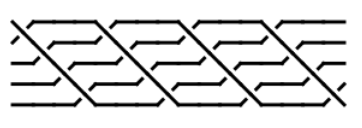
\includegraphics[width=0.7\textwidth]{braid_diagram}
  \caption{Example of a braid diagram}\label{fig:braid_diagram}
\end{figure}



\subsection{Quandles generalize coloring}

A $p$ coloring of a knot diagram $d \in \diag(K)$ is a mapping $C: \A(d) \to Z_p$

\subsection{Deriving the quandle axioms from the Reidemeister moves}
\label{sec:quandle_axioms}


\begin{figure}[h]
  \centering
  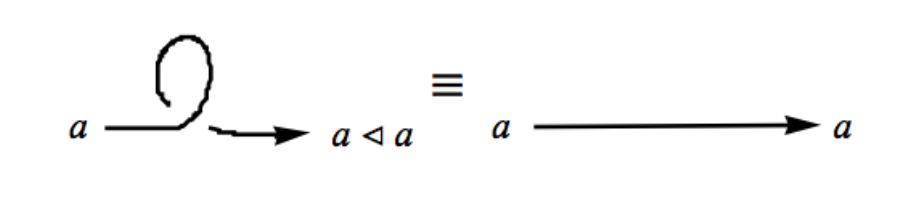
\includegraphics[width=0.8\textwidth]{R1}
  \caption{R1. Figure reproduced from~\cite{Cusick}}\label{fig:r1}
\end{figure}

\begin{figure}[h]
  \centering
  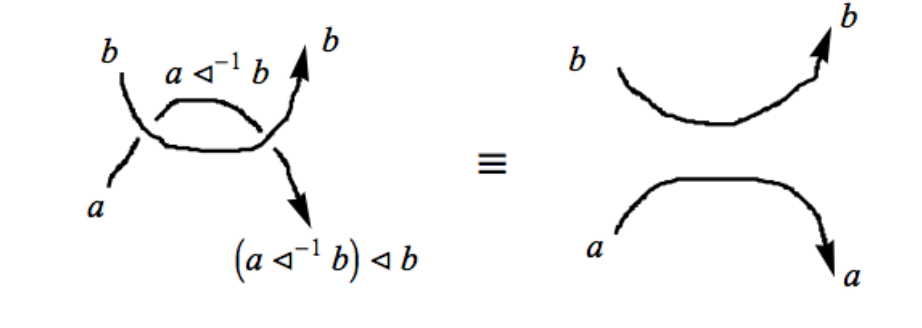
\includegraphics[width=0.8\textwidth]{R2}
  \caption{R2. Figure reproduced from~\cite{Cusick}}\label{fig:r2}
\end{figure}

\begin{figure}[h]
  \centering
  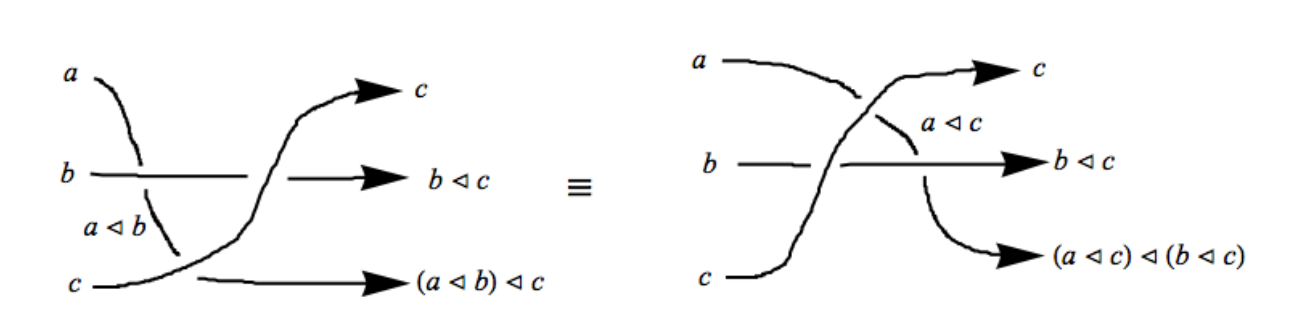
\includegraphics[width=0.8\textwidth]{R3}
  \caption{R3. Figure reproduced from~\cite{Cusick}}\label{fig:r3}
\end{figure}



\subsection{Involutary Quandle}
In this paper we concern ourselves with \textbf{Involutory Quandles}. An \textbf{involutory quandle} is any set $K$ equiped with a binary operation $\uc$ that satisfies $3$ axioms:

\begin{equation}
	x \uc x = x
\end{equation}
\begin{equation}
	x \uc (x \uc y) = y \\
\end{equation}
\begin{equation}
	x \uc (y \uc z) = (x \uc y) \uc (x \uc z) \\
\end{equation}

These equations can be though of a symbolic representations of Reidemeister moves. $(1)$ corresponds to the Type I Reidemeister move, $(2)$ corresponds to the Type II Reidemeister move, and $(3)$ corresponds to the Type III Reidemeister move. (See Fig)

\subsection{Alexander Quandle}

The \textbf{Alexander Quandle} is defined as:

$$ x \uc y = ty + (1 - t)a $$

$t$ is usually a free variable in $\mathbb{C}$ however for this paper we consider a special case of the Alexander Quandle:

$$ x \uc y = qy + (1 - q)a $$

where $q$ is a free variable in $\mathbb{Z}_n$. The reasons for this will be made clear when we consider the relationship between the Alexander Quandle and coloring.

\subsection{Dihedral Quandle}
The \textbf{Dihedral Quandle} is defined as:

$$x\uc y = 2x - y$$

it is a special case of the Alexander quandle when $t$ is evaluated at $-1$.

\subsection{Coloring}

We say that a knot $K$ is $Z_p$ colorable if given an prime $p > 2$ every strand in the projection of $K$ can be labeled using numbers $0$ to $p-1$, with at least 2 of the labels distinct so that at each crossing we have:

$$ 2x - y - z = 0 \mod p $$

(TODO: Cite FinalPaper.pdf)

\subsection{Quandle Coloring}

We say that a knot $K$ is $Z_{p,q}$ colorable if for some unit $q \in \mathbb{Z}_p$ every strand in the projectio of $K$ can be labeled using numbers $0$ to $p-1$ such that at each crossing we have:

$$qx - (1-q)y - z \equiv 0 \mod p $$ 

\end{document}
